\documentclass[letterpaper,11pt]{article}

\usepackage[T1]{fontenc}
\usepackage[utf8]{inputenc}
\usepackage{graphicx}
\usepackage{xcolor}
\usepackage{color}
\usepackage{pdflscape}
\usepackage{forest}

\renewcommand\familydefault{\sfdefault}
\usepackage{tgheros}
\usepackage[defaultmono]{droidmono}

\usepackage{amsmath,amssymb,amsthm,textcomp}
\usepackage{enumerate}
\usepackage{multicol}
\usepackage{tikz}


\usepackage{geometry}
\geometry{total={210mm,297mm},
left=25mm,right=25mm,%
bindingoffset=0mm, top=20mm,bottom=20mm}


\linespread{1.3}

\newcommand{\linia}{\rule{\linewidth}{0.5pt}}

% custom theorems if needed
\newtheoremstyle{mytheor}
    {1ex}{1ex}{\normalfont}{0pt}{\scshape}{.}{1ex}
    {{\thmname{#1 }}{\thmnumber{#2}}{\thmnote{ (#3)}}}

\theoremstyle{mytheor}
\newtheorem{defi}{Definition}

% my own titles
\makeatletter
\renewcommand{\maketitle}{
\begin{center}
\vspace{2ex}
{\huge \textsc{\@title}}
\vspace{1ex}
\\
\linia\\
\@author \hfill \@date
\vspace{4ex}
\end{center}
}
\makeatother
%%%

% custom footers and headers
\usepackage{fancyhdr}
\pagestyle{fancy}
\lhead{}
\chead{}
\rhead{}
\lfoot{LT Homework 1}
\cfoot{}
\rfoot{Page \thepage}
\renewcommand{\headrulewidth}{0pt}
\renewcommand{\footrulewidth}{0pt}
%

% code listing settings
\usepackage{listings}

\lstset{language=Python,
    aboveskip={1.0\baselineskip},
    belowskip={1.0\baselineskip},
    columns=fixed,
    extendedchars=true,
    breaklines=true,
    tabsize=4,
    prebreak=\raisebox{0ex}[0ex][0ex]{\ensuremath{\hookleftarrow}},
    frame=lines,
    showtabs=false,
    showspaces=false,
    showstringspaces=false,
    keywordstyle=\color{blue},
    stringstyle=\color{red},
    commentstyle=\color{green},
    morecomment=[l][\color{magenta}]{\#},
    numbers=left,
    numberstyle=\small,
    stepnumber=1,
    numbersep=10pt,
    captionpos=t,
    escapeinside={\%*}{*)}
}

%%%----------%%%----------%%%----------%%%----------%%%

\begin{document}

\title{LT Homework 1}

\author{Gavin Fynbo --- U54777118}

\date{24 October, 2017}

\maketitle

\section*{Note}
\em All programs were written in \textbf{Python 3.6} and all directions for running and getting results from the source code can be found in the \textbf{README.md} file included in the directory. \em
\section*{Problem 1}
\textbf{Solution:}\\
(a)\\
What's included here is the CDF of the $1,000$ randomly generated values. The program can be seen in the attached file \textbf{part1.py} and the graph of the values is shown as it was generated by \em matplotlib\em .\\
\\
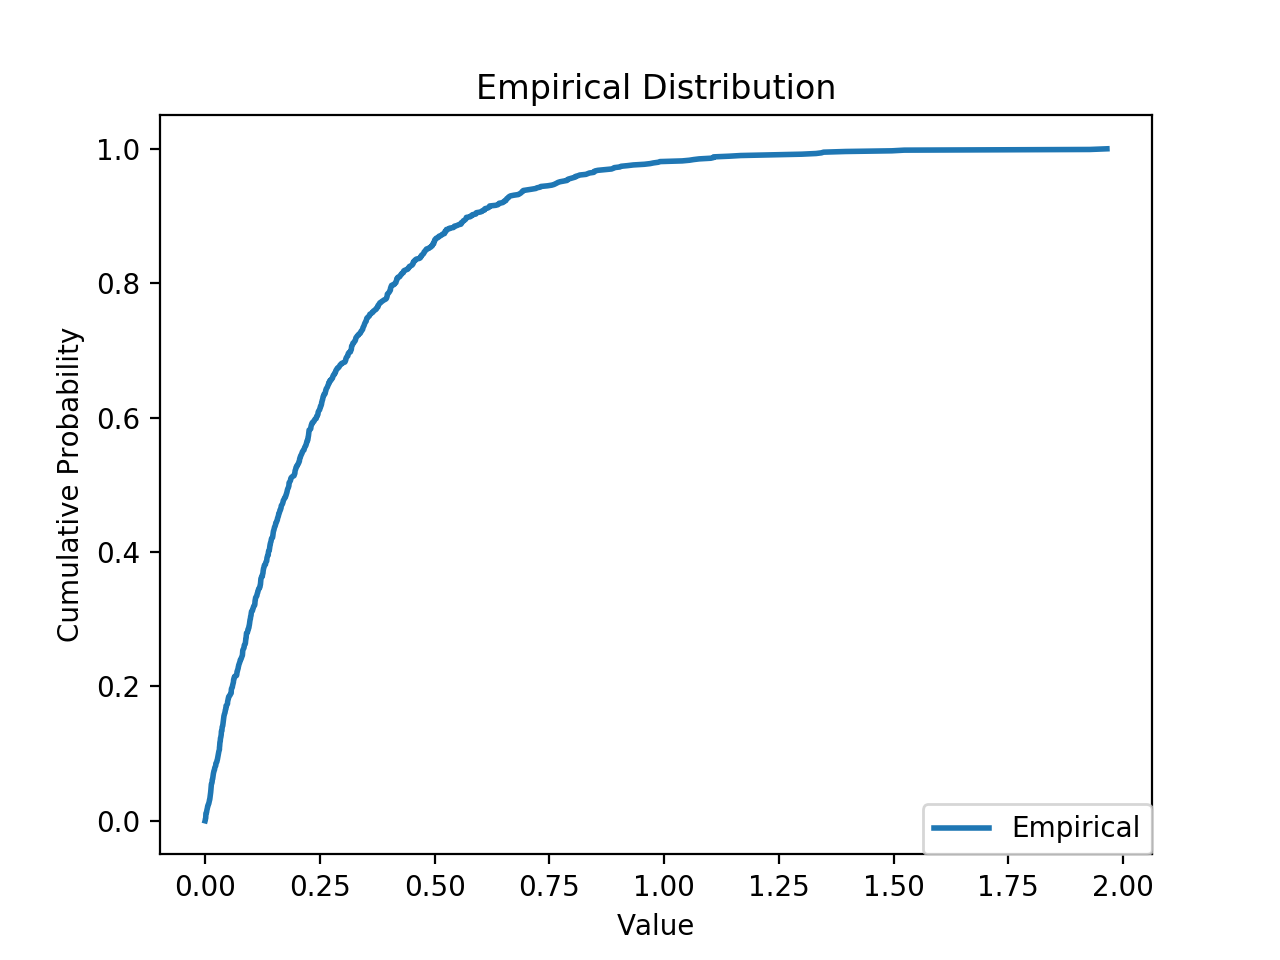
\includegraphics[scale=1]{Empirical.png}\\
\\
(b)\\
What I have done for the second part is generate the Empirical graph as before, but also overlay the Analytical graph on top of it to give a sense of the accuracy of the program. They do not match exactly because the Analytically generated portion of the graph will follow the function exactly whereas the Empirically generated portion is only going to become closer and closer given a larger number of samples. However, given the size of our sample we get a close approximation to the actual formula.\\
\\
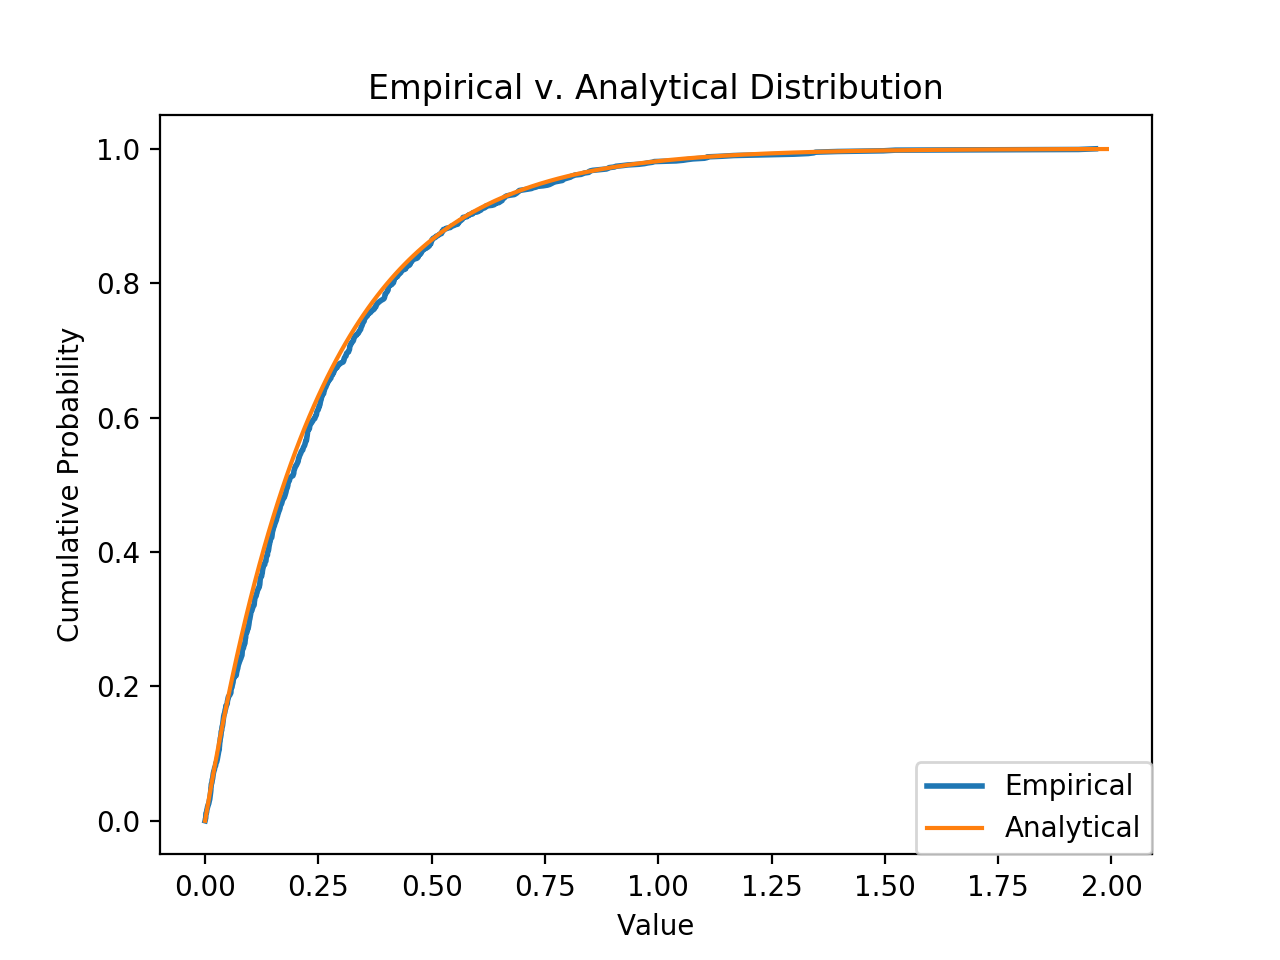
\includegraphics[scale=1]{Empirical-v-Analytical.png}\\
\\

\section*{Problem 2}
\textbf{Solution:}\\
(a)\\
The program is written in Python 3 in this directory under the name \textbf{part2.py} and can be run via the command line as "python3 part2.py L T S" where L, T, and S stand for $\lambda$, $T_s$, and simulation time respectively. Additionally, if you need to see how to put in the commands enter "python3 part2.py -h".\\
The results of the monitor events can be seen in the generated file in the same root directory under the name \textbf{monitor\_results.txt}.\\
(b)\\
For $\lambda = 5;\ T_s = 0.15;\ sim\_time = 1000$ we get the following:\\
$q = $ the number of average customers in the system, which we can approximate by taking exponentially distributed random times under $\lambda = 1$ and creating a list and then taking the mean or average of that list.\\
Additionally, these numbers were calculated after the system had time to "warm up", meaning that it was allowed to reach a steady state and then we calculated the numbers to get a more accurate representation. The calculations are as follows:\\
$queue\_mean = $ this stat is measured by the monitor event in the system in addition to $lam\_mean$ and $ts\_mean$ by compiling a list and deriving the averages.\\
$util = (1 / lam\_mean) * ts\_mean$\\
$q = queue\_mean + (util)$\\
$T_q = q / (1 / lam\_mean)$\\
$T_w = queue\_mean / (1 / lam\_mean)$\\
\\
$$T_w = 0.4437\ seconds.$$
$$T_q = 0.5883\ seconds.$$
$$w = 2.2174\ customers/requests.$$
$$q = 2.9400\ customers/requests.$$
$$\rho = 0.7226$$
(c)\\
An analytical calculation of this M/M/1 system with Little's Law would give us the following results:\\
$$T_w = 0.45\ seconds.$$
$$T_q = 0.60\ seconds.$$
$$w = 2.25\ customers/requests.$$
$$q = 3.00\ customers/requests.$$
$$\rho = 0.75$$
This means that all of our simulated system is very close to the analytical representation we are seeing in a mathematically calculated M/M/1 system. Thus, it is a good representation of the system.\\
(d)\\
These are the empirical measurements:\\
$$T_w = 1.3340\ seconds.$$
$$T_q = 1.1890\ seconds.$$
$$w = 7.1893\ customers/requests.$$
$$q = 8.1020\ customers/requests.$$
$$\rho = 0.9127$$
vs.\\
An analytical calculation of this M/M/1 system with Little's Law would give us the following results:\\
$$T_w = 1.35\ seconds.$$
$$T_q = 1.50\ seconds.$$
$$w = 8.10\ customers/requests.$$
$$q = 9.00\ customers/requests.$$
$$\rho = 0.90$$
The system is still fairly accurate but the queuing numbers are a little low, still a good representation however.\\
(e)\\
These are the empirical measurements:\\
$$T_w = 247.65\ seconds.$$
$$T_q = 247.85\ seconds.$$
$$w = 1524.95\ customers/requests.$$
$$q = 1526.15\ customers/requests.$$
$$\rho = 1.209$$
vs.\\
An analytical calculation of this M/M/1 system with Little's Law would give us the following results:\\
$$T_w = inf\ seconds.$$
$$T_q = inf\ seconds.$$
$$w = inf\ customers/requests.$$
$$q = inf\ customers/requests.$$
$$\rho = 1.20$$
We can see here that because of utilization of greater than $\rho > 1$ we have infinitely increasing queues and wait times.\\

\section*{Problem 3}
\textbf{Solution:}\\
(a)\\
See attached source code for \textbf{part3.py}.\\
(b)\\
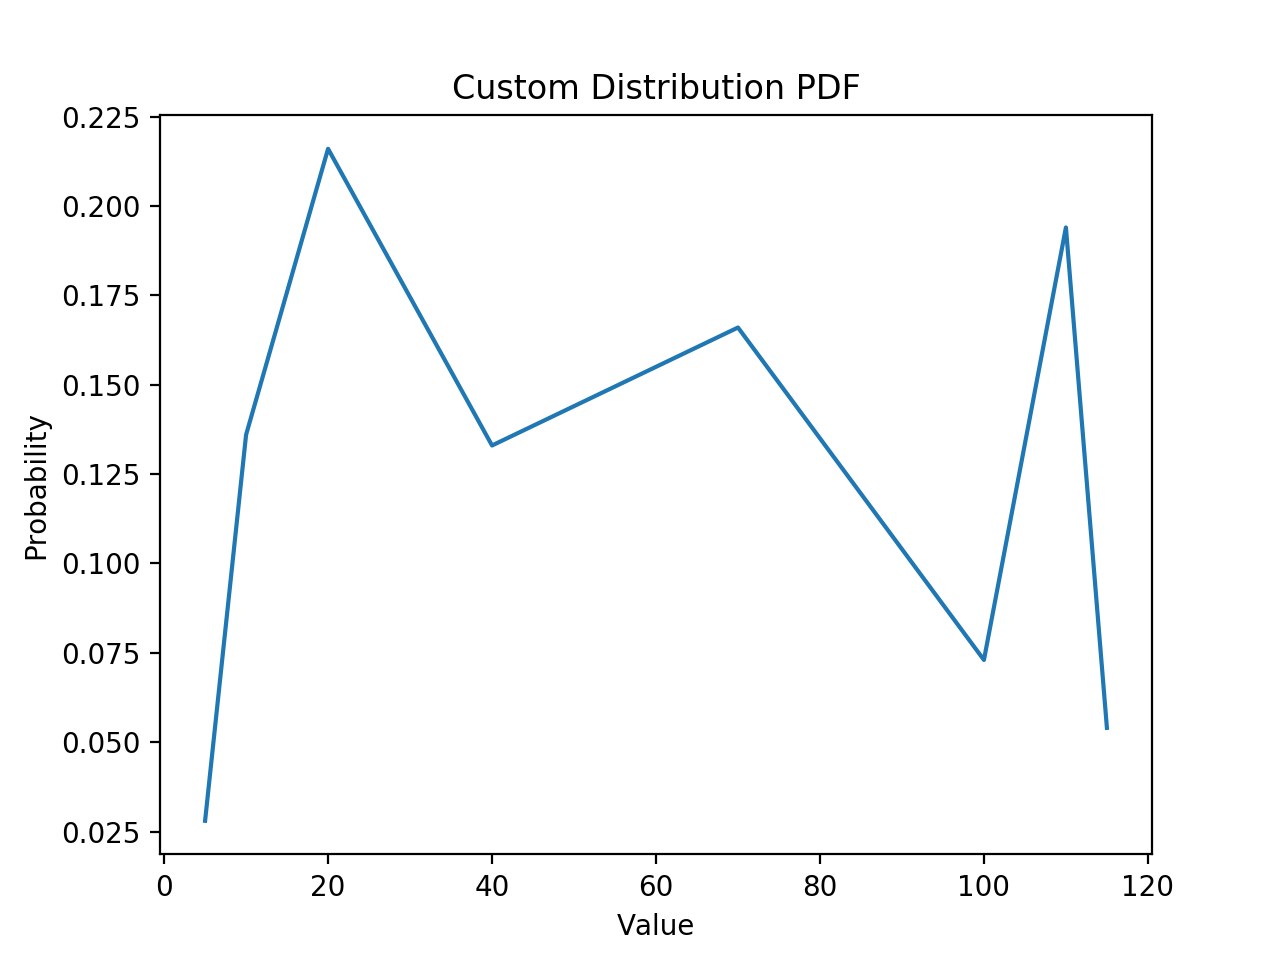
\includegraphics[scale=1]{Custom-Dist.png}\\
(c)\\ 
The outcomes are nearly identical to the properties that were defined in the given table. This means that the custom distribution is functioning correctly, it practically simulates the distribution, but with some variation due to randomness.\\

\section*{Problem 4}
\textbf{Solution:}\\
(a)\\
The program is written in Python 3 in this directory under the name \textbf{part4.py} and the key to modeling this system is to use a series of M/M/1 queues via Jackson's Theorem to model and simulate the system. This also means we can steal the majority of our code from Part 2. Using Jackson's Theorem we can assume that given the server is at a steady state that the rate of arrivals between all M/M/1 systems is $\lambda$.\\
\\
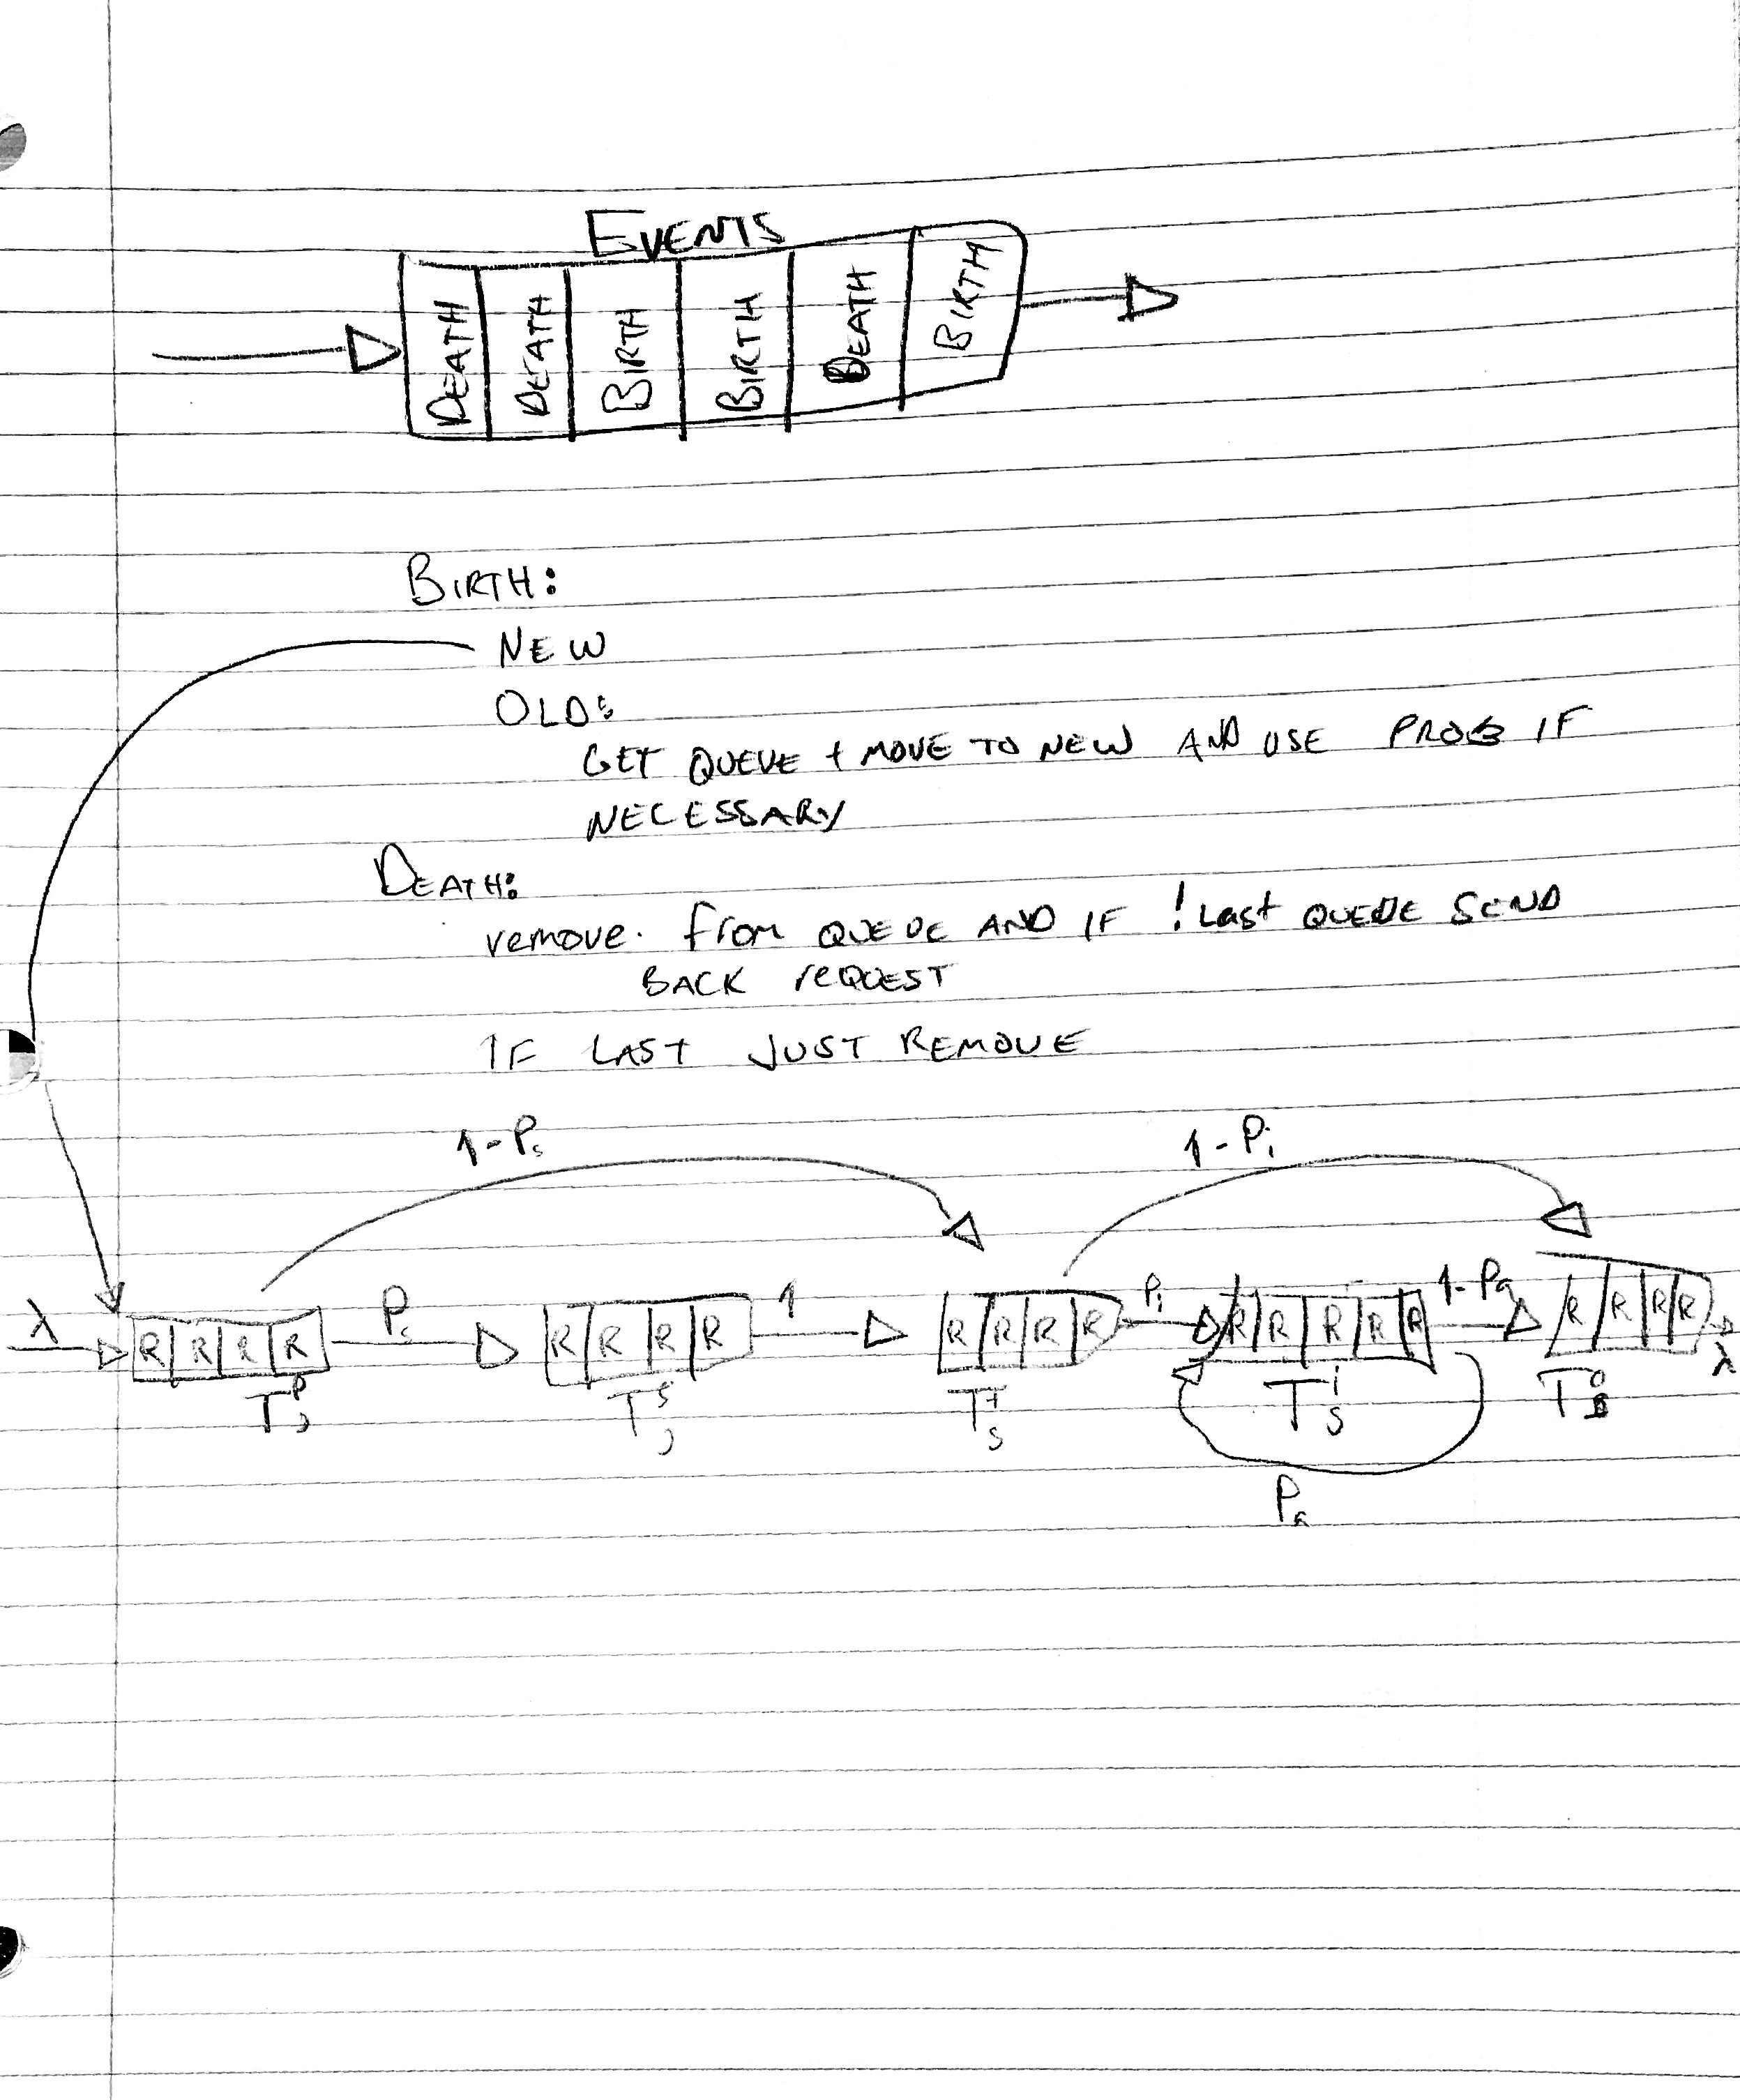
\includegraphics[scale=0.2]{Diagram.jpg}\\
\\
(b)\\
Using a monitor event I kept track of the average service times in each queue in the whole system and using that and Jackson's Theorem I can calculate the utilization of each queue in the system. These are calculated using the program.\\
$$\rho(T_s^p) = 0.049$$
$$\rho(T_s^s) = 0.099$$
$$\rho(T_s^f) = 1.204$$
$$\rho(T_s^i) = 0.464$$
$$\rho(T_s^o) = 0.119$$
(c)\\ 
Given the various utilizations I can say that the bottleneck is the reading the required file from the disk as it exceeds or approaches $100\%$.\\
(d)\\
There is a bottleneck.\\
(e)\\
The throughput of the disk is simply the number $N$ of requests serviced in a give time $T$ with a rate of $H$. In this case $N = 19789$, $T = 2000$ and $\frac{19789}{2000} = 9.89\ requests/sec$.\\
(f)\\
In this case we can take the total departures of the interpreter divided by the percentage of the time it was used out of the total time to get the throughput of the interpreter.\\
$$\frac{7717}{0.35 * 2000} = \frac{7717}{700} = 11.024\ requests/sec$$

\end{document}


